\section{Event Storming}\label{sec:event-storming}
In diesem Unterkapitel werden die grundlegenden Prinzipien und Ziele des \ac{DDD} erläutert, welche von Vaughn Vernon in seinem Buch
\textit{Domain-Driven Design Distilled} definiert hat.\cite*{dddd}
Nachdem diese Grundlage vorhanden ist, wird darauf aufbauend erklärt, welche Symbiose aus dem \ac{DDD} und dem \ac{ES} entsteht und wie
dies zu einer Softwareentwicklung beiträgt.
Abschließend werden die Änderungen und Erweiterungen, welche im Kontext dieser Arbeit vorgenommen wurden, erklärt.

\subsection{Domain-Driven Design}\label{subsec:domain-driven-design}
Das \ac*{DDD} ist nicht nur für die erste Phase der Softwareentwicklung praktisch, sondern ebenso für das Umstrukturieren bestehender Projekte.
Ein grundlegendes Ziel des \ac{DDD} ist es ein Projekt in sogenannte \textit{Bounded Contexts} zu unterteilen und damit zu umgehen, dass
die Anwendung aus einem riesigen aufgeblähten Modell besteht.
Um dieses Ziel zu erreichen, ist es wichtig in Gesprächen mit Domänenexperten die wichtigsten Punkte eines \textit{Bounded Context} zu evaluieren.
Domänenexperten können in jedem Bereich eines Unternehmens gefunden werden.
Es ist nötig ein möglichst breites Spektrum an Personen zu haben, um den gesamten zu entwickelnden Prozess zu verstehen und für die Entwickler verständlich zu machen.
Dabei ist es wichtig, dass alle Personen, welche am Prozess des \ac{DDD} teilnehmen eine einheitliche Sprache zu entwickeln.
Diese einheitliche Sprache beschreibt Vernon als~\textit{Ubiquitous Language}.\footnote{Seite 7 in~\cite*{dddd}}
Eine allgegenwärtige Sprache (\textit{Ubiquitous Language}) zu entwickeln, ist ein fortlaufender Prozess.
Initial ist es wichtig, dass zwischen den verschiedenen Domänenexperten und den Entwicklern diese einheitliche Sprache entsteht, welche
nicht nur das Verständnis zwischen den beiden Parteien, sondern auch mit in das Modell einfließen soll.

\subsection{Event Storming}\label{subsec:allgemein}
Vernon selbst nennt Event Storming, als eine Möglichkeit um eine~\textit{Ubiquitous Language} zu entwickeln.\footnote{Seite 112, folgende in~\cite*{dddd}}
Event Storming wurde von Alberto Brandolini entwickelt und resultiert aus mangelnder Zeit während der Nutzung von~\textit{event-driven modeling}.
\textit{Event-driven modeling} basiert ebenfalls auf Konversationen und konkreten Szenarien, allerdings mit der Verwendung von UML-Diagrammen zur Datenmodellierung.
Dies hatte zur Konsequenz, dass in Gesprächen ab einem bestimmten Punkt nur noch die Entwickler daran teilnahmen.
Brandolini verwarf UML-Diagramme und verwendete Haftnotizen und legte damit für das~\ac{ES}.\footnote{Seite 113 in~\cite*{dddd}}

In seinem Buch, \textit{Introducing EventStorming}, beschreibt Brandolini mehrere Event Storming Workshops und wie diese durchgeführt wurden.\cite*{introES}
Hierbei stellt sich heraus, dass Event Storming kein starres Konstrukt aus Abläufen ist, sondern je nach Kontext angepasst werden kann.
Dennoch gibt es Ähnlichkeiten, welche eine solide Grundlage für ein Event Storming Workshop bieten.\footnote{Seite 23 in~\cite*{introES}}
Neben einem grenzenlosen Platz zum Modellieren benötigt es genügend Marker und Haftnotizen in verschiedenen Formen und Farben.
Die teilnehmenden Domänenexperten benötigen eine kollaborative Einstellung zur Modellierung, ein offenes Miteinander ungeachtet ihrer Stellung.
Keine Grenzen zu dem Thema oder der Anwendung welche modelliert werden soll, um weitere Probleme oder Fragen zu lösen und beantworten zu können.
Ein Event Storming beginnt immer mit dem Erstellen von Domain Events und dem Platzieren dieser anhand eines Zeitstrahles.
Zudem müssen alle Beteiligten am fortlaufenden Verfeinern eines Modells interessiert sein, da ein \ac{ES}-Workshop zum Lernen und Verbessern
von Anwendungen gedacht ist.
Ein Event Storming Board\footnote{\url{https://www.softwarecraftsperson.com/2021/04/25/event-storming/}}
nach einem solchen Workshop ist in Abbildung~\ref{fig:rlBoard} dargestellt.

\begin{figure}[ht]
    \centering
    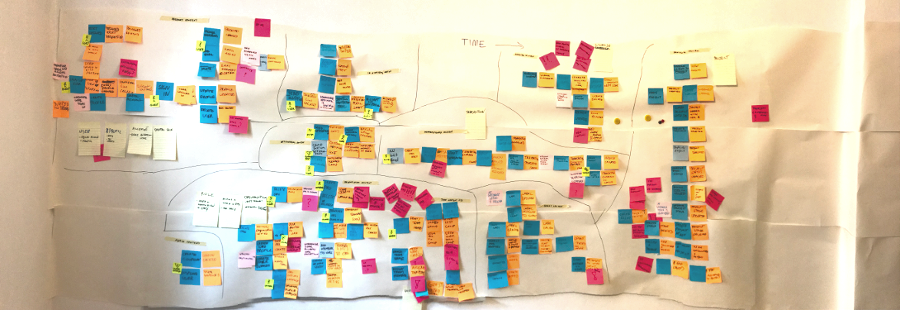
\includegraphics[width=0.75\textwidth]{images/2.1/event-storming}
    \caption{Event Storming Board}
    \label{fig:rlBoard}
\end{figure}

Nachdem initial Domain Events beim \ac{ES} erstellt wurden, soll jedem ein Command vorausgesetzt werden.
Ein Command fungiert hierbei als die Aktion, welche das Event ausgelöst hat.
Dies können Aktionen eines Nutzers oder externen Systems sein.
Während eines Workshops können sogenannte \textit{Hotspots} in Gesprächen entdeckt werden.
Dabei kann es sich um Probleme aber auch Fragen bezüglich des Ablaufs handeln, welche wichtig für die spätere Anwendung werden.

Wie auch das~\ac{DDD} kann Event Storming jederzeit während des Entwicklungsprozesses verwendet werden.
Für die verschiedenen Anwendungsbereiche hat Brandolini mehrere Typen des Event Stormings definiert.
Hierbei bleibt die Methodik an sich die gleiche, allerdings wird das Ziel genauer definiert.\newline
\textbf{Big Picture EventStorming} wird während eines Kick-off Meetings eingesetzt, damit alle Teilnehmer den Inhalt und den Bereich der zur erstellenden Anwendung kennenlernen.
Hierzu ist es nötig, dass alle Interessengruppen vertreten sind, welche innerhalb des Unternehmens existieren und ebenfalls eine Entscheidungsgewalt innehaben.\newline
\textbf{Design Level EventStorming} findet auf einer tieferen Ebene einen Einsatz.
Dabei handelt es sich um das Erstellen möglicher Implementierungen, zum Beispiel, ob Event Sourcing oder andere Techniken aus dem~\ac{DDD} verwendet werden sollen.
Es werden somit Entscheidungen getroffen, welcher in erster Linie die Entwickler betrifft und von diesen am besten zu bewerten ist.\newline
\textbf{Value-Driven EventStorming} bietet einen Einstieg in die Wertstromanalyse (englisch: value-stream mapping).
Anhand einer solchen Analyse ist es möglich den Erhalt von Informationen und der Verarbeitung dieser darzustellen und Probleme zu erkennen.\newline
\textbf{UX-Driven EventStorming} konzentriert sich auf das Erlebnis eines Nutzers/Kunden bei der Benutzung der Anwendung.
Hierbei wird neben der Nutzerfreundlichkeit auch die fehlerfreie Ausführung abgebildet und überprüft.\newline
\textbf{EventStorming as a Retrospective} konzentriert sich darauf einen Ablauf über Domain Events zu definieren und nach
Erweiterungsmöglichkeiten zu suchen, welche Vorteile für die Anwendung bereitstellen können.\newline
\textbf{EventStorming as a Learning Tool} zeigt auch die weiteren Lernchancen innerhalb eines Unternehmens.
Mittels Event Storming ist es somit auch möglich neue Angestellte möglichst schnell auf den aktuellen Stand zu bringen.
Diese Art von Lernchancen ist ebenfalls im~\textbf{Big Picture EventStorming} enthalten.

\subsection{Erweiterung}\label{subsec:erweiterung}
\todo{Hier das vorherige Kapitel abwarten um alle Änderungen/Erweiterungen besser daran fest zu machen.}
\begin{itemize}
    \item Erweiterungen für Wirtschaft (Pages -> daraus generierte Mockups, abgehen von dem "Wir wollen keinen PC benutzen" des ES)
    \item Ideen für die Lehre (Wird in dieser Arbeit nicht näher beleuchtet, da es für den Beleg der Funktionalität nicht mehr möglich ist dies ausreichend in der Bearbeitungszeit zu machen)
    \item ES -> Ablauf von Schritten -> Albert -> Workflow (Arbeitsablauf) beschreibungen -> Mögliche Idee zum besseren Nahebringen von komplexeren Abläufen in Vorlesungen. (Verbildlichung)
\end{itemize}
